% Created 2016-07-13 mié 21:51
\documentclass[11pt,letterpaper]{article}
\usepackage[T1]{fontenc}
\usepackage{fixltx2e}
\usepackage{graphicx}
\usepackage{grffile}
\usepackage{longtable}
\usepackage{wrapfig}
\usepackage{rotating}
\usepackage[normalem]{ulem}
\usepackage{amsmath}
\usepackage{textcomp}
\usepackage{amssymb}
\usepackage{capt-of}
\usepackage{hyperref}
\usepackage{minted}
\usepackage{xltxtra}
\usepackage[top=2.0cm, bottom=3cm, left=2.0cm, right=2.0cm]{geometry}
\author{Juan Ávalo, Bastien Got}
\date{\today}
\title{Tarea 3 Análisis Inteligente de Datos}
\hypersetup{
 pdfauthor={Juan Ávalo, Bastien Got},
 pdftitle={Tarea 3 Análisis Inteligente de Datos},
 pdfkeywords={},
 pdfsubject={},
 pdfcreator={Emacs 25.1.50.2 (Org mode 8.3.4)}, 
 pdflang={English}}
\begin{document}

\maketitle
\tableofcontents


\section{Reconocimiento de Texto}
\label{sec:orgheadline3}
El problema de ésta parte es reconocer si un comentario de un sitio web de
películas es favorable o desfavorable.
\subsection{Preprocesamiento de los datos.}
\label{sec:orgheadline1}
\begin{enumerate}
\item Tanto el set de entrenamiento como el de pruebas tienen \textbf{3554} datos.
Los datos se separan en textos positivos y negativos de acuerdo a la tabla:
\begin{center}
\begin{tabular}{|c|c|c|}
\hline
Sets & Positivos & Negativos\\
\hline
Entrenamiento & 1770 & 1784\\
Prueba & 1803 & 1751\\
\hline
\end{tabular}
\end{center}
\item Se creó una función que extrae palabras usando \emph{stemming} y quitando
\emph{stopwords} si así es pedido. Sobre los resultados obtenidos se puede
observar con los ejemplos usados que \emph{stemming} lo que hace es hacer que
una palabra tome una pseudoraiz. Además, el proceso de quitar \emph{stopwords}
efectivamente quita palabras como "I" o "to".

Como ejemplo, las frases: "I love to eat cake" y "I love eating cake" ambas
se reducen a "love", "eat" y "cake".

Pero un ejemplo más interesante es el de aplicar \emph{stemming} sobre palabras
como "absolutely" y "dislike", las cuales se traducen en "absolut" y
"dislik". Ninguna de las pseudoraices es una palabra del inglés verdadera,
pero van a ser útiles para saber que palabras están relacionadas o no.
\item También se creó una función análoga a la del punto anterior, pero
lematizando. Para poder lograr ésto no se pudo usar la función
\texttt{WordNetLemmatizer} directamente como estaba en los ejemplos.

Lematización involucra hacer un análisis sintáctico de las palabras, por lo
que la función usada pide marcar cada palabra con la posición dentro de la
oración que tiene (verbo, sustantivo, adjetivo, adverbio), la cual se
obtuvo mediante la función \texttt{pos\_tag}.

Los efectos en las palabras de ejemplo son aparentes. En casos como el de
"I love to eat cake" el lematizador las reduce de la misma forma que usando
\emph{stemming}. La diferencia se nota al usar las palabras "dislike" y
"absolutely", las cuales se mantienen iguales. O con palabras como "are" e
"is" las cuales se reducen a "to be".
\item Se generaron cuatro representaciones vectoriales para los dos conjuntos de
datos. La razón de ésto es porque se necesita extraer palabras con
\emph{stemming} y con \emph{lemmatize}, con \emph{stopwords} y sin ellas.

La representación del texto consiste en resumir cada comentario a un vector
binario con todo el vocabulario obtenido de todos los mensajes. Si el
mensaje tiene una palabra dentro del vocabulario, el valor de la variable
correspondiente a esa palabra es \textbf{1}. Sino es \textbf{0}. 

Luego las etiquetas son \textbf{0} si el mensaje es negativo, y \textbf{1} si es
positivo.

Considerando como se tratan los datos, se puede rankear las palabras que
globálmente se encontraron por frecuencia. Un ejemplo de ello es la
siguiente tabla:

\begin{center}
\begin{tabular}{|c|c|}
\hline
Frecuencia & Palabra\\
\hline
115 & way\\
125 & get\\
127 & well\\
128 & much\\
129 & work\\
143 & even\\
143 & time\\
145 & comedy\\
163 & character\\
169 & good\\
176 & story\\
246 & one\\
254 & like\\
264 & make\\
481 & movie\\
573 & film\\
\hline
\end{tabular}
\end{center}
\item El evaluador de desempeño considera las siguientes medidas:
\begin{itemize}
\item La precisión del modelo sobre los datos de entrenamiento.
\item La precisión del modelo sobre los datos de prueba.
\item La \emph{precisión}, esto es, el porcentaje de datos bien clasificados dentro de
todos los datos clasificados.
\item El \emph{recall} el cual es el porcentaje de los datos seleccionados bien
clasificados dentro de los datos de su clase.
\item El \emph{f1-score}, el cual es la media armónica entre la precisión y el
recall.
\item El support, que cuenta cuantos datos de cada clase hay.
\end{itemize}
\end{enumerate}
\subsection{Modelos a probar.}
\label{sec:orgheadline2}
Al dataset procesado mediante las combinaciones de stemming, lemmatize y
stopword removal se le aplicaron cuatro modelos de clasificación: "Naive
Bayes", "Multinomial Naive Bayes", "Logistic Regression" y "Linear SVC". 

En general los resultados eran prácticamente todos con un f1-score mayor a
0.70. Se notó en general que, sobre el comportamiento de las predicciones,
éstas eran más certeras mientras más vocabulario asociado a textos favorables
o desfavorables tenían. 

Ninguno de los tipos de modelo se comporta bien con frases sarcásticas o con
críticas que tienen muchas palabras que en otro contexto serían positivas.

Casi todos los modelos entregaban, a parte de la predicción concreta, un par
de valores que corresponde a la probabilidad de que el texto sea positivo o
negativo. Si ambos valores se parecían, indica que el modelo no tiene certeza
de que clase de texto es. Por otro lado, si uno de los valores es muy grande
indica una casi absoluta certeza en el resultado.

Los resultados generales para todos los modelos son resumidos por el
siguiente gráfico, tomando como medida el mayor f1-score obtenido por cada
modelo.
\begin{figure}[htb]
\centering
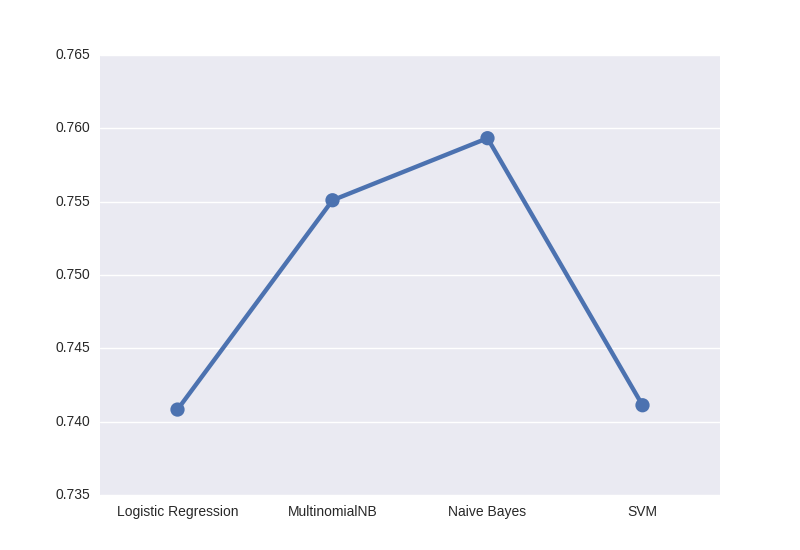
\includegraphics[width=0.6\textwidth]{p2_general.png}
\caption{Resultados generales.}
\end{figure} 

Curiosamente, el modelo más simple con la menor cantidad de preprocesamiento
es la que resulto mejor evaluada usando la métrica de f1-score y los modelos
más complicados resultaron peor evaluados. 

Viendo más en detalle, los resultados para los distintos modelos se
encuentran en los siguientes gráficos. El resumen para todos ellos es que
las predicciones son mejores mientras menos preprocesamiento haya.

En el caso del uso de \emph{stopwords} se asume que las palabras que son omitidas
mediante éste paso, para efectos de clasificar sí son importantes. Dejar de
lado palabras como "I" puede cambiar el contexto de la frase y con esto
cambiar el sentimiento que se quería transmitir.

Sobre la lematización se puede atribuir los problemas a dificultades en
obtener los \emph{tags} semánticos apropiados para cada palabra, más el hecho de
que los comentarios de internet de por si pueden tener palabras que no están
en el diccionario de WordNetLemmatizer, por lo cual no descubriría relaciones
que stemming si encuentra. 

\begin{figure}[H]
\centering
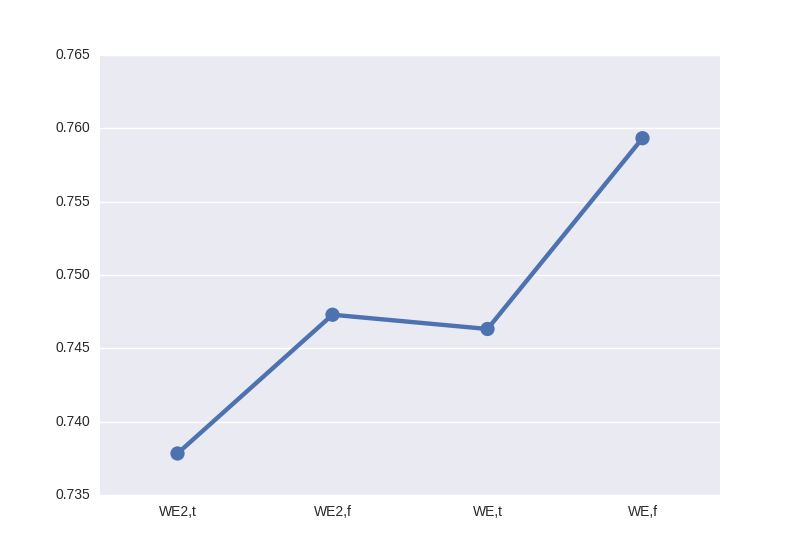
\includegraphics[width=0.6\textwidth]{p2_f1_naive.png}
\caption{\emph{Naive Bayes}.}
\end{figure} 


\begin{figure}[H]
\centering
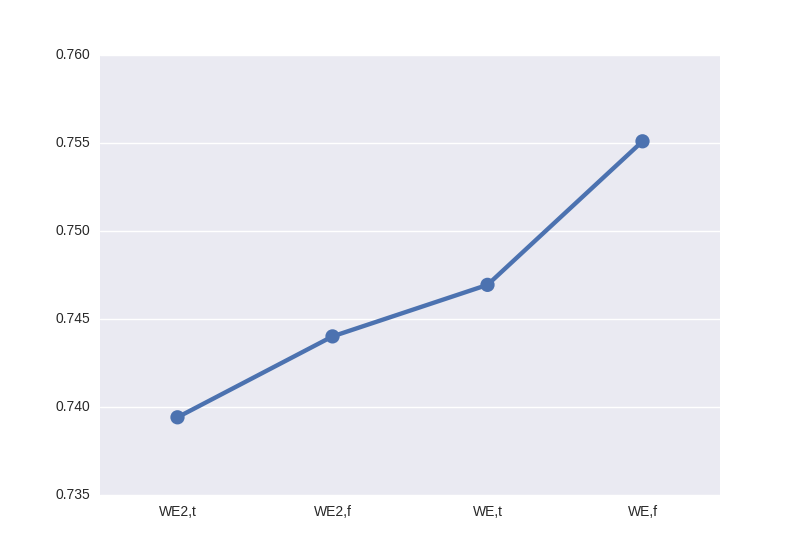
\includegraphics[width=0.6\textwidth]{p2_f1_multinomial.png}
\caption{\emph{multinomial naive bayes}.}
\end{figure} 


\begin{figure}[H]
\centering
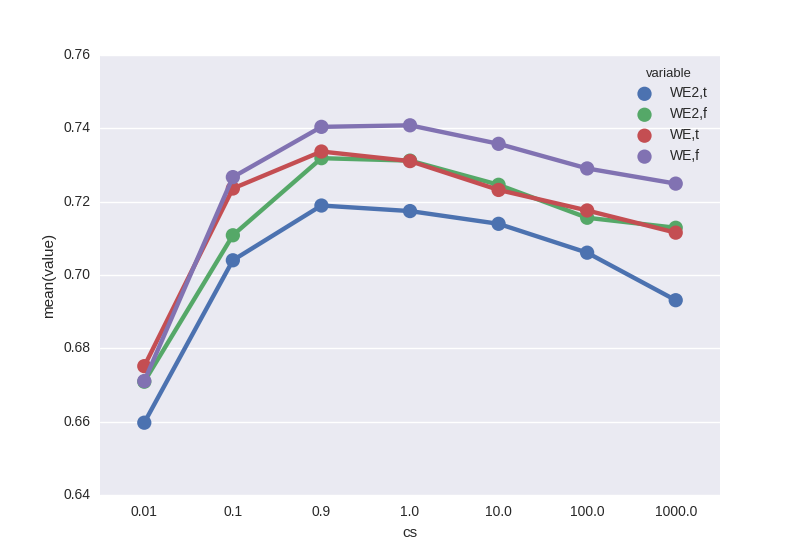
\includegraphics[width=0.6\textwidth]{p2_f1_logit.png}
\caption{\emph{Logistical Regression}.}
\end{figure} 


\begin{figure}[H]
\centering
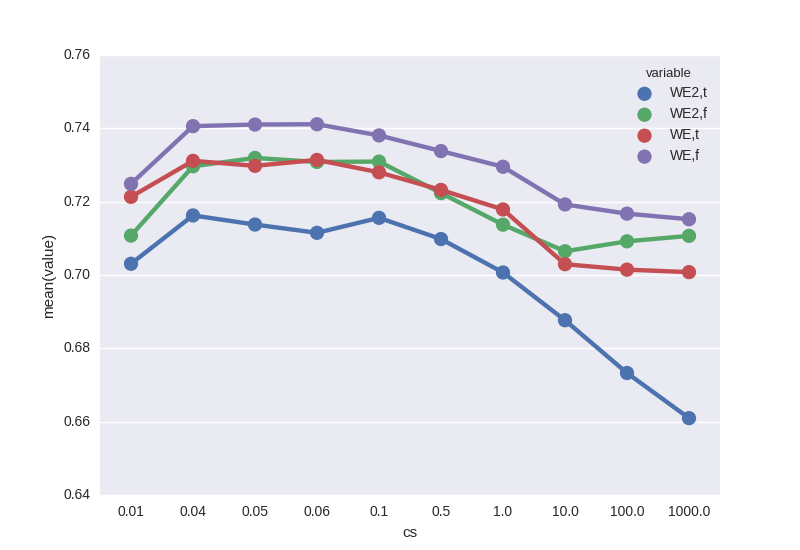
\includegraphics[width=0.6\textwidth]{p2_svm_logit.png}
\caption{\emph{Linear SVM}.}
\end{figure} 

Hay que hacer ciertas observaciones al respecto del parámetro \texttt{C} de
\emph{Logistical Regression} y \emph{Linear SVM}. Los gráficos anteriores muestran
valores aproximados de los mejores parámetros que se pueden elegir, los
cuales son \(C_{logit} = 0.9\) y \(C_{svm} = 0.05\). 

Además, analizando los valores de las probabilidades de obtener un label en
cada texto escogido por la función de test, se puede ver en el caso de
\emph{Logistical Regression} que aumentar \texttt{C} hace que las predicciones sean mas
determinantes. O sea, el modelo resultante tiene menos dudas al momento de
decidir a que label le corresponde cada texto. Viceversa si \texttt{C} disminuye,
para efectos del modelo los textos parecen ser más ambiguos. 

Usando la función \emph{Linear SVM} no se puede saber si el modelo resultante
sigue la misma tendencia con las probabilidades, ya que no son entregadas por
la función correspondiente. Usando \emph{SVM} con un kernel lineal, lo cual
debería ser equivalente salvo detalles de implementación, permite encontrar
las probabilidades, las cuales siguen el mismo patrón.
\end{document}